\section{Background}  \label{Background}

This section establishes the thesis's foundation by reviewing essential concepts, beginning with Autonomous Driving Systems (ADS). It utilizes the SAE J3016 standard~\cite{sae:j3016:2021apr} to define ADS, its automation levels, and critical safety requirements such as Dynamic Driving Task (DDT) performance during failures and DDT Fallback to a minimal risk condition, while also covering challenges like sensor failures and non-deterministic software, and their mitigation strategies. The section then examines Video Object Detection (VOD), a crucial perception task for ADS, outlining its evolution from basic frame-by-frame detection to sophisticated techniques leveraging temporal data, including post-processing, motion-information-based approaches (e.g., RNNs, LSTMs), feature filtering (e.g., attention mechanisms), and top-performing Transformer-based models. Finally, the General Purpose Perceiver model is introduced, detailing its architecture and novel cross-attention mechanism that allows it to process diverse, high-dimensional inputs by first projecting them into a smaller latent space, thereby addressing traditional Transformer scaling issues, paving the way for the thesis's proposed architectural modifications for enhanced sequential data processing relevant to these domains.

\subsection{Autonomous Driving Systems} \label{Background:AutonomousDrivingSystems}

% thesis: Autonomous Driving Systems have high safety requirements.

The Society of Automotive Engineers (SAE) International's J3016 standard \cite{sae:j3016:2021apr} establishes a comprehensive framework for Autonomous Driving Systems. SAE J3016 \cite{sae:j3016:2021apr} defines an Autonomous Driving System (ADS) as the hardware and software collectively capable of performing the entire Dynamic Driving Task (DDT) on a sustained basis. The DDT encompasses all real-time operational and tactical functions requisite for on-road vehicle operation. It is important to note that SAE specifically employs the term 'ADS' to describe automation systems at Level 3, Level 4, or Level 5 of driving automation \ref{fig:figure_background_j3016_levels_of_driving_automation}.

\begin{figure}
    \centering
    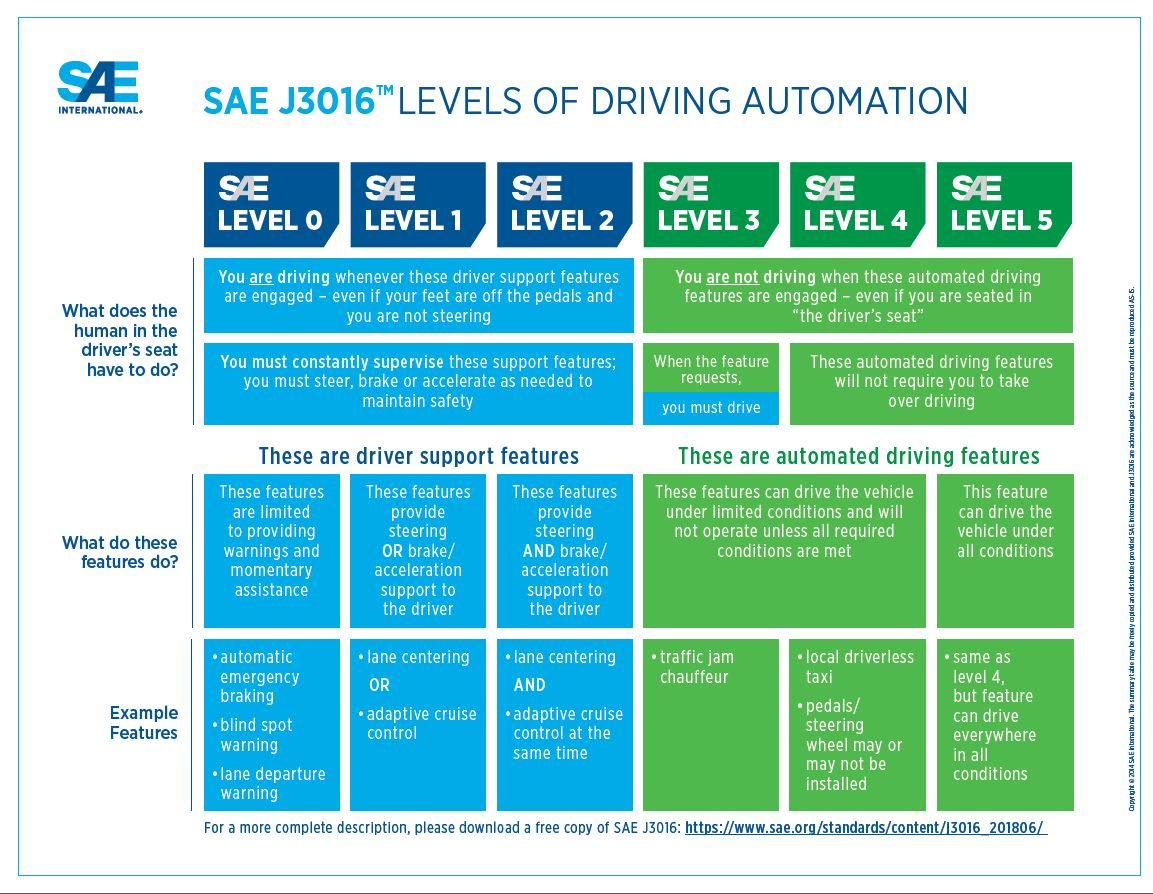
\includegraphics[width=\textwidth]{figures/figure_background_j3016_levels_of_driving_automation.jpg}
    \caption{Levels of Driving Automation. This figure illustrates the six levels of driving automation as defined by the SAE J3016 standard, ranging from no automation (Level 0) to full vehicle autonomy (Level 5). The graphic clarifies the role of the human driver at each level and provides examples of corresponding driver support and automated driving features \cite{sae:j3016:2021apr}.}
    \label{fig:figure_background_j3016_levels_of_driving_automation}
\end{figure}

SAE J3016 \cite{sae:j3016:2021apr} stipulates stringent safety requirements for ADS, particularly concerning their operational behavior during DDT performance-relevant system failures and the subsequent execution of the DDT Fallback. DDT Fallback refers to the response by the user or the ADS to either perform the DDT or achieve a minimal risk condition following such a system failure. A minimal risk condition, as defined by the standard, is a stable, stopped condition to which a user or an ADS may bring a vehicle after performing the DDT fallback in order to reduce the risk of a crash when a given trip cannot or should not be continued. The standard defines these safety expectations, including the management of DDT Fallback and the achievement of a minimal risk condition, differently for each automation level.

For Level 3 Conditional Driving Automation, a key mandate of SAE J3016 \cite{sae:j3016:2021apr} is that in the event of a system failure, the ADS, after issuing an intervention request to the designated fallback-ready user, is obligated to continue performing the DDT for a duration of several seconds. This capability to maintain DDT performance for a critical period after the request underscores the system's operational capacity under failure and provides the necessary transition time. This temporal window is intended to afford the fallback-ready user, who is expected to be vigilant and prepared, sufficient time to assess the situation and either resume vehicle control or transition the vehicle to a minimal risk condition, should they ascertain its necessity. A presumption within the standard is that the fallback-ready user will be receptive to such intervention requests and to conspicuous system failures.

In contrast, Level 4 High and Level 5 Full Driving Automation are subject to more stringent safety requirements, a core aspect of which is their mandatory capability to perform the complete DDT Fallback under a performance-related system failure. These advanced systems must autonomously execute this fallback procedure and attain a minimal risk condition independently of human intervention. Consequently, Level 4 and 5 systems are designed to autonomously address failures and ensure vehicle safety, for example, by maneuvering to a roadside stop.

A foundational principle articulated by SAE for ADS pertains to their inherent operational resiliency—specifically, their capacity to maintain safe operations amidst system failures. At Level 3, this resiliency manifests through an orchestrated human-machine interaction, which ensures the user is afforded adequate time to resume control. Conversely, for Levels 4 and 5, resiliency implies that the ADS autonomously executes the fallback procedure and transitions the vehicle to a minimal risk condition. These safety-critical functionalities are deemed indispensable for fostering public trust and facilitating the extensive and safe deployment of autonomous driving technologies.

% goal: present two types of failures relevant to the thesis

The operational scope of an Autonomous Driving System (ADS) is defined by its Operational Design Domain (ODD). The ODD specifies the precise conditions under which a given ADS is designed to function reliably. These conditions encompass a wide range of factors, including, but not limited to, roadway types, geographical constraints, speed limitations, and environmental conditions \cite{sae:j3016:2021apr}.

Broadly, ADS architectures are categorized into two principal approaches: modular and end-to-end \cite{tampuuSurveyEndtoEndDriving2022}, both architectures are shown in the Figure \ref{fig:figure_background_ads_system_architecture}. The modular approach, also termed the mediated perception approach and considered conventional, organizes the driving task into a series of interconnected, self-contained modules such as perception, localization, planning, and control \cite{tampuuSurveyEndtoEndDriving2022}. Conversely, end-to-end driving, sometimes referred to as behavior reflex, conceptualizes the entire pipeline—from processing sensory inputs to generating vehicle control commands (e.g., steering, acceleration)—as a singular, learnable machine learning task, often actualized through a unified neural network \cite{tampuuSurveyEndtoEndDriving2022}. Irrespective of the architectural approach, ADSs are equipped with a comprehensive suite of sensors to construct a detailed model of their environment. This sensor suite commonly includes cameras, LiDAR (light detection and ranging), radar, and ultrasonic sensors \cite{matosSurveySensorFailures2024}. Recognizing that sensors vary in technology and purpose, each with inherent weaknesses, necessitates sensor fusion—the combination of inputs from multiple sensors—to overcome these individual limitations, reduce errors, and thereby achieve a consistent, accurate, and robust perception of the environment \cite{matosSurveySensorFailures2024}.

\begin{figure}
    \centering
    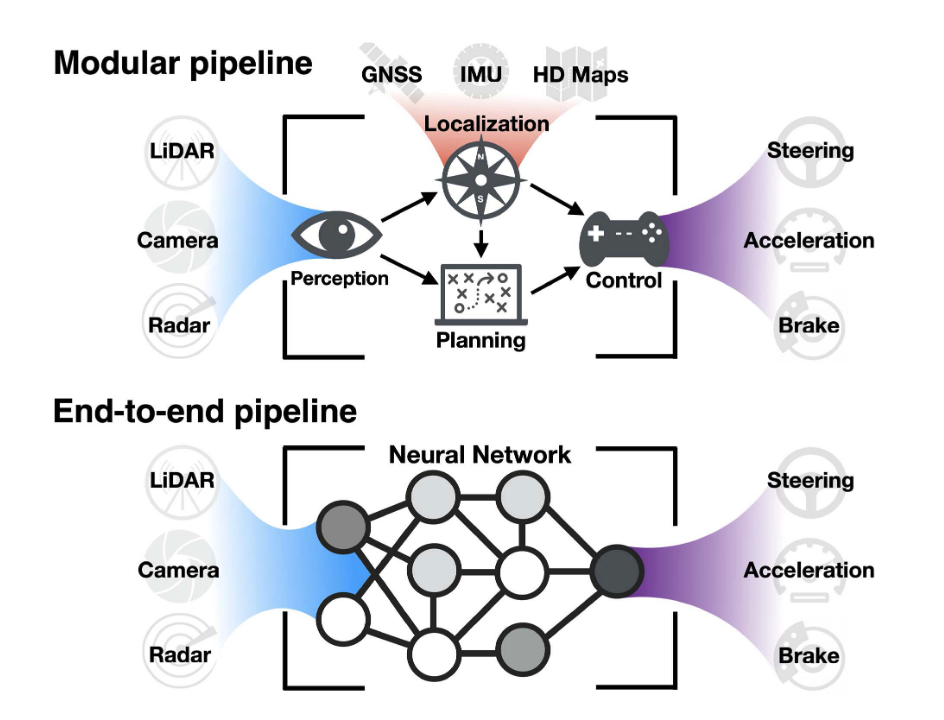
\includegraphics[width=\textwidth]{figures/figure_background_ads_system_architecture.png}
    \caption{Modular and end-to-end pipelines. The modular pipeline for autonomous driving consists of many interconnected modules, whereas the end-to-end approach treats the entire pipeline as one learnable machine learning task \cite{tampuuSurveyEndtoEndDriving2022}.}
    \label{fig:figure_background_ads_system_architecture}
\end{figure}

Given the reliance on a complex sensor suite and operation in diverse environments, the potential for sensor failures presents a significant challenge in ADS design and validation. Sensor failures can manifest in various forms, from partial degradation of performance under adverse environmental conditions—such as cameras being affected by glare or low light, or LiDAR and RADAR performance being impacted by heavy precipitation—to the complete malfunction of a sensor unit \cite{matosSurveySensorFailures2024}. While a core design objective is to prevent catastrophic system failure, the occurrence of individual sensor faults or the degradation of a specific sensing modality is a credible event that the ADS must be engineered to handle gracefully. Key mitigation strategies include advanced sensor fusion algorithms, which intelligently combine data from disparate sensor sources to enhance accuracy and compensate for the limitations or failure of any single sensor. In instances of complete failure of a critical sensor or an entire sensor modality, redundancy is the primary mitigation strategy.

The ADS's computational hardware and software stack processes data streams generated by its diverse sensor array. Integrating and fusing this data presents a fundamental challenge due to different sensors inherently operating at varying sampling rates, possessing different internal processing latencies, and being subject to communication delays. Temporal calibration, which involves accurately timestamping and synchronizing these heterogeneous data streams, is a mitigation strategy that can address aspects of this non-deterministic behavior to some extent \cite{matosSurveySensorFailures2024}. The software systems integral to ADSs, often employing middleware like the Robot Operating System (ROS) or its real-time focused iteration ROS 2.0 for inter-process communication and data synchronization. Traditional middleware such as ROS 1.0 was not originally architected for stringent real-time performance, and its underlying mechanisms can introduce variability in message latencies and task execution times \cite{parkRealTimeCharacteristicsROS2020}. While newer frameworks like ROS 2.0 aim to enhance real-time performance and determinism using technologies such as the Data Distribution Service (DDS) \cite{parkRealTimeCharacteristicsROS2020}, achieving complete elimination of non-deterministic behavior in these large-scale distributed software systems remains exceptionally challenging. Therefore, despite mitigation strategies like temporal calibration and advancements in middleware, non-deterministic software behavior remains an issue.


% goal: explain relevance between sensors and video object detection task

The Dynamic Driving Task (DDT), as defined by SAE J3016, encompasses all real-time operational and tactical functions required for on-road vehicle operation \cite{sae:j3016:2021apr}. These functions include lateral and longitudinal vehicle motion control, as well as monitoring the driving environment. A critical set of subtasks of the DDT is Object and Event Detection and Response (OEDR). OEDR involves the subtasks of monitoring the driving environment (detecting, recognizing, and classifying objects and events, and preparing to respond as needed) and executing an appropriate response to complete the DDT \cite{sae:j3016:2021apr}. It is the system's capability to perform the entire DDT, including OEDR, that distinguishes an ADS (Levels 3-5) from lower-level driving automation system. The perception aspect of OEDR is also known as perception and a variety of computer vision tasks fall under this category, such as object detection, semantic segmentation, 3D object detection, and others \cite{yurtseverSurveyAutonomousDriving2020}.

To fulfill the stringent safety requirements articulated for Autonomous Driving Systems, notably by standards such as SAE J3016 \cite{sae:j3016:2021apr}, it is imperative that ADSs are designed and validated to be resilient against the aforementioned failures, including complete sensor failure and the impacts of non-deterministic software behavior. This thesis contributes to addressing these challenges by proposing specific training procedures and evaluation protocols. These are designed to simulate and rigorously assess perception model robustness and its potential for ADS.

\subsection{Video Object Detection} \label{Background:VideoObjectDetection}

% Object detection definition. Deep learning pushed performance of single image object detection.

%TODO: add more exampleas of the progress in CV (from Object Detection from Video Tubelets with Convolutional Neural Networks)
Object detection is a foundational challenge in computer vision and has been a subject of research for several decades \cite{fischlerRepresentationMatchingPictorial1973}. The goal of the object detection task is to find objects of a given description in images and videos.
Advancements in deep learning techniques for feature representation learning \cite{hintonReducingDimensionalityData2006, lecunDeepLearning2015}, in conjunction with the significant development and application of deep Convolutional Neural Networks (CNN), have driven remarkable progress in various computer vision tasks, such as image classification \cite{krizhevskyImageNetClassificationDeep2012}, object detection \cite{girshickRichFeatureHierarchies2014a}.
Extending detection capabilities from static images to video sequences introduces the task of video object detection, which involves not only localizing objects within each frame but also leveraging temporal information across frames for improved accuracy and consistency.
The introduction of specific challenges, such as the video object detection track in the ImageNet Large Scale Visual Recognition Challenge (ILSVRC) \cite{russakovskyImageNetLargeScale2015}, provided benchmark datasets and standardized evaluation protocols, significantly accelerating research and development in the video object detection domain.

% State-of-the-Art
% Still-image detector
Due to the inherent similarity between detecting objects in single images and in video frames, the most straightforward approach to video object detection task is to apply a single-image object detector independently to each frame. 
This method, often referred to as frame-by-frame detection, treats each frame as independent image. %TODO: add citation where it's refered as f-to-f
However, such an approach ignores the rich temporal and contextual information available across consecutive video frames. Neglecting this temporal dimension often leads to suboptimal performance, characterized by issues like inconsistent bounding box predictions across frames, flickering detections, and reduced robustness to challenges specific to video, such as motion blur, occlusion, morphological diversity, and illumination variations within the video \cite{jiaoNewGenerationDeep2022}. 
Consequently, while applying static detectors frame-by-frame serves as a simple baseline, it is generally not considered an effective or optimal solution for the complexities of video object detection. %TODO: Add citation with examples

% For example, if an object is detected in neighboring frames but not in the current frame, we can recover the missing object in the current frame by applying temporal coherence.
% Another example is that mistakenly-labeled objects can be corrected by checking the semantic labels across the frames.

Video object detection algorithms can be broadly classified based on their architectural solution to the video object detection task. For this thesis, the classification proposed by the survey \cite{jiaoNewGenerationDeep2022} is adopted. This survey categorizes these algorithms into four main types: those based on image detection (postprocessing methods), those utilizing motion information (introducing additional models), those employing feature filtering, and other effective network structures.

\begin{figure}
    \centering
    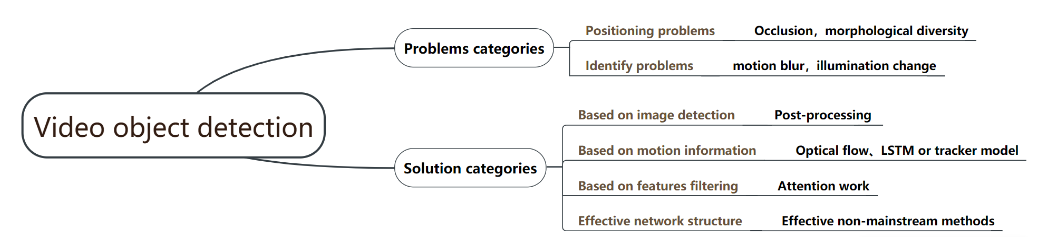
\includegraphics[width=\textwidth]{figures/figure_background_vod_classification.png}
    \caption{Classification of video object detection problems and solutions \cite{jiaoNewGenerationDeep2022}.}
    \label{fig:figure_background_vod_classification}
\end{figure}

% Postprocessing (not e2e)
% T-CNN: ImageNet VID 2015 73 - 77 mAP
One strategy involves applying a postprocessing step to the outputs of a still-image detector to enhance temporal consistency \cite{hanSeqNMSVideoObject2016, kangTCNNTubeletsConvolutional2018, kangObjectDetectionVideo2016}. This often utilizes detections from adjacent frames to refine the results for the current frame. Common postprocessing techniques include Sequence Non-Maximum Suppression (Seq-NMS), which links high-scoring detection boxes across frames into sequences \cite{hanSeqNMSVideoObject2016}, or leveraging optical flow to propagate detection scores \cite{kangTCNNTubeletsConvolutional2018, kangObjectDetectionVideo2016}. While these methods can improve upon static image detectors, exploiting temporal information solely during postprocessing is considered suboptimal, as crucial temporal and motion cues are disregarded during the primary detector training phase. Therefore, such algorithms have difficulty overcoming consecutive failures of the static image detector when the object of interest experiences long-term occlusions or significant appearance changes.

% motion information

To address the limitation of postprocessing, another category of methods utilizing motion information by introducing additional models to integrate motion and temporal information directly into the model training, often creating end-to-end solutions. This category is subdivided into models based on optical flow, contextual information, and trajectory information. For the purpose of this thesis, a subcategory of contextual information is reviewed, which utilizes Recurrent Neural Networks (RNN) and their variants. The power of RNNs in long-range temporal representation has become a valuable tool for the video object detection task \cite{Lu_2017_ICCV, xiaoVideoObjectDetection2018, liuMobileVideoObject2018}, enabling the design of end-to-end networks. One of the challenges posed by such methods is how to associate objects within the RNN structure across multiple frames.

One notable early attempt to tackle this association problem is the Association LSTM framework \cite{Lu_2017_ICCV}. The framework consists of an SSD image detector \cite{liuSSDSingleShot2016} and a variant of the RNN model, the Long Short-Term Memory (LSTM) network \cite{6795963}. SSD detects frame-wise, image-based object detection results (bounding box, score, and object feature) which are stacked and fed into the LSTM. The association LSTM not only regresses and classifies directly on object locations and categories but also associates features to represent each output object. By minimizing the matching error between these features, the network learns how to associate objects in two consecutive frames. Additionally, the method works in an online manner, which is important for real-world applications. The authors acknowledge that a weakness of these frameworks is that the LSTM module is a post-hoc addition, since performance is limited by the quality of the initial SSD detections. Missed or poorly localized detections by the SSD are difficult for the LSTM to recover. Furthermore, the SSD parameters are not updated during training.

% T-CNN with LSTM
% TUBELETS: ImageNet VID 2015 ~75ish mAP

% % STMN: ImageNet VID 2015 80.5 mAP
Building upon the idea of modeling temporal dependencies but aiming for deeper integration and leveraging spatial information more effectively, the Spatial-Temporal Memory Network (STMN) was proposed \cite{xiaoVideoObjectDetection2018}. Unlike the Association LSTM which operates on vector-form features within a standard LSTM, STMN introduces a Spatial-Temporal Memory Module (STMM). This module utilizes a modified bidirectional convolutional Gated Recurrent Unit (ConvGRU) \cite{ballasDelvingDeeperConvolutional2016}, allowing it to process and retain information in a spatially structured manner directly from convolutional feature maps generated by the detector backbone. By preserving spatial locality within the recurrent computation, STMM can better capture appearance changes and motion patterns. Experimental results indicated that the effectiveness of such convolutional memory modules increases with the length of the input sequence, as more relevant long-range context can be accumulated, leading to improved detection accuracy, particularly for challenging scenarios involving occlusion or significant appearance variations \cite{xiaoVideoObjectDetection2018}.

The principle of using convolutional recurrent units to efficiently propagate spatio-temporal information proved beneficial not only for accuracy but also for enabling real-time video object detection on resource-constrained platforms. In this work \cite{liuMobileVideoObject2018}, an architecture is introduced that augments a single-image object detector (SSD with a pruned MobileNet base) by interweaving efficient convolutional LSTM (ConvLSTM) \cite{shiConvolutionalLSTMNetwork2015} layers, specifically "Bottleneck-LSTM" layers, to refine and propagate feature maps across frames. Despite its more complex architecture, an array of modifications is proposed that allow this model to be faster and more lightweight than mobile-focused single-frame models.

% Feature filtering

Another category of video object detection methods employs feature filtering techniques to enhance performance by selectively focusing on relevant spatiotemporal information while suppressing redundant or irrelevant data. This approach draws inspiration from the human visual system, which can rapidly identify salient regions within a scene, thereby optimizing cognitive resources for efficient analysis \cite{ittiModelSaliencybasedVisual1998}. Similarly, feature filtering mechanisms in neural networks aim to prioritize critical features and reduce unnecessary computations, leading to improvements in both accuracy and efficiency \cite{jiaoNewGenerationDeep2022}. These methods can be broadly subdivided based on the specific filtering mechanism employed, notably attention mechanisms \cite{bahdanauNeuralMachineTranslation2016a, vaswaniAttentionAllYou2023} and deformable convolutions \cite{daiDeformableConvolutionalNetworks2017a}.

Attention mechanisms allow networks to dynamically weigh the importance of different features or spatial locations across video frames. This selective focus enables the propagation of crucial information, particularly for objects undergoing significant appearance changes or movements, potentially offering advantages over methods relying solely on adjacent frame correlations or optical flow, which can struggle with large displacements and add significant model complexity \cite{jiaoNewGenerationDeep2022, guoProgressiveSparseLocal2019}.

One prominent example is the Progressive Sparse Local Attention (PSLA) framework \cite{guoProgressiveSparseLocal2019}. Addressing limitations associated with optical flow, such as increased model size and difficulty handling large displacements or high-level features, PSLA provides an alternative mechanism for establishing feature correspondence and propagating information between frames \cite{guoProgressiveSparseLocal2019}. Instead of calculating pixel-level flow, PSLA operates directly on feature maps. While similar to STMN \cite{xiaoVideoObjectDetection2018} which also uses local correlation for alignment, PSLA differs by utilizing a sparse neighborhood and softmax normalization for better spatial correspondence, aiming to improve both speed and accuracy \cite{guoProgressiveSparseLocal2019}. It uses a special attention approach called progressive sparse stride, which pays more attention to nearby features (for small movements) and less attention to features farther away (for larger movements). By calculating weighted correspondences based on feature similarity within this sparse local neighborhood, PSLA aligns and aggregates features across time, enabling temporal feature updating and enhancement without relying on an explicit optical flow model. This approach aims to achieve a better balance between accuracy, speed, and model size compared to traditional flow-based methods \cite{guoProgressiveSparseLocal2019}. Nevertheless, managing the complexity of attention calculations remains a factor.

The final category outlined by \cite{jiaoNewGenerationDeep2022}, termed "Other Effective Network Structures", incorporates a range of exploratory and innovative methodologies for video object detection. While Transformer-based approaches were not explicitly itemized under this classification in the \cite{jiaoNewGenerationDeep2022} survey, the author of this thesis has taken the considered step of including them within this category. This decision is predicated on an analysis of their architectural principles and their significant subsequent impact on the field, which aligns with the innovative spirit of the "Other Effective Network Structures" designation. Prominent among these emergent architectures are those predicated on the Transformer model \cite{vaswaniAttentionAllYou2023}. Initially transformative within the domain of natural language processing, the Transformer architecture has subsequently exhibited considerable promise for applications in computer vision, most notably in the task of object detection \cite{carionEndtoEndObjectDetection2020}.

Pioneering works like Detection Transformer (DETR) \cite{carionEndtoEndObjectDetection2020} reformulated object detection as a direct set prediction problem. To address some of the initial limitations of DETR, such as slow convergence and high computational cost, Deformable DETR \cite{zhuDeformableDETRDeformable2021} was introduced. It incorporates a deformable attention module that only attends to a small set of key sampling points around a reference, significantly improving efficiency and performance. However, the encoder in early DETR variants was identified as a computational bottleneck, a point highlighted in subsequent research such as \cite{linD^2ETRDecoderOnlyDETR2022}.

Building on these foundational image-based object detection Transformers, researchers began adapting them for the complexities of video. Subsequent adaptations for the video domain have demonstrated considerable success, with DETR-based methodologies achieving high performance. A notable example specifically designed for video is TransVOD \cite{zhouTransVODEndtoEndVideo2023}. TransVOD constructs an end-to-end Video Object Detection framework utilizing a spatial-temporal Transformer. This architecture is designed to effectively detect objects and maintain their identities by modeling relationships across frames, thus tracking how objects move and change throughout a video sequence. Further advancements in this domain include models like PTSEFormer (Pyramidal Temporal-Spatial Encoder Transformer) \cite{wangPTSEFormerProgressiveTemporalSpatial2022}, which introduces a novel pyramidal temporal-spatial encoder. This encoder aims to efficiently capture multi-scale spatio-temporal features by progressively integrating information from different temporal and spatial resolutions, enhancing the model's ability to handle variations in object scale and motion.

The impact of these Transformer-based models is underscored by their strong performance on established benchmarks. Indeed, Transformer-based methods are among the top-scoring approaches in challenges such as the ImageNet VID (Video Object Detection) task \cite{russakovskyImageNetLargeScale2015}. Their inherent ability to model long-range dependencies and learn complex spatio-temporal relationships positions them as a critical area of ongoing research and development in the field of video object detection.

\subsection{General Purpose Perceiver Model} \label{Background:Perceiver}

Most architectures used by AI systems today are specialized. For instance, models presented in \ref{Background:VideoObjectDetection} built for the video object detection task might excel at processing 2D video frames, but they are hardly ideal for other data types, such as the LiDAR point clouds or radar output used in ADS. Handling multiple data modalities, like the sounds and images that make up videos, presents even greater complexity and usually involves complex, hand-tuned systems built from many different parts, even for simple tasks. Real-world problems, such as building an ADS, possess these complexities, so there is a desperate need to build a simple yet effective, more general, and versatile architecture that can handle all types of data.

Perceiver \cite{jaeglePerceiverGeneralPerception2021} was introduced as a general-purpose architecture that is capable of processing different data types such as images, point clouds, audio, video, and, what is important, combinations of those to fuse together. The Perceiver builds upon the Transformer \cite{vaswaniAttentionAllYou2023}, an architecture that uses an operation called "Attention" to map inputs into outputs \cite{bahdanauNeuralMachineTranslation2016a}. While attention is simple and widely applicable, the way Transformers utilize attention can become memory expensive as the number of inputs grows. Consequently, Transformers perform well with inputs containing at most a few thousand elements, but common data forms like images and videos can easily comprise millions of elements. This fact poses a challenge to the generalist architecture: scaling the Transformer's attention operation to very large inputs without introducing domain-specific assumptions. The Perceiver addresses this by using attention to first encode the inputs into a small latent array. This latent array can then be processed further at a cost independent of the input's size, allowing the Perceiver's memory and computational needs to scale gracefully as the input size grows, even for particularly deep models. This "graceful growth" enables the Perceiver to achieve an unprecedented level of generality - it is competitive with domain-specific models on benchmarks based on images, 3D point clouds, and combined audio and images \cite{jaeglePerceiverGeneralPerception2021}.

\begin{figure}
    \centering
    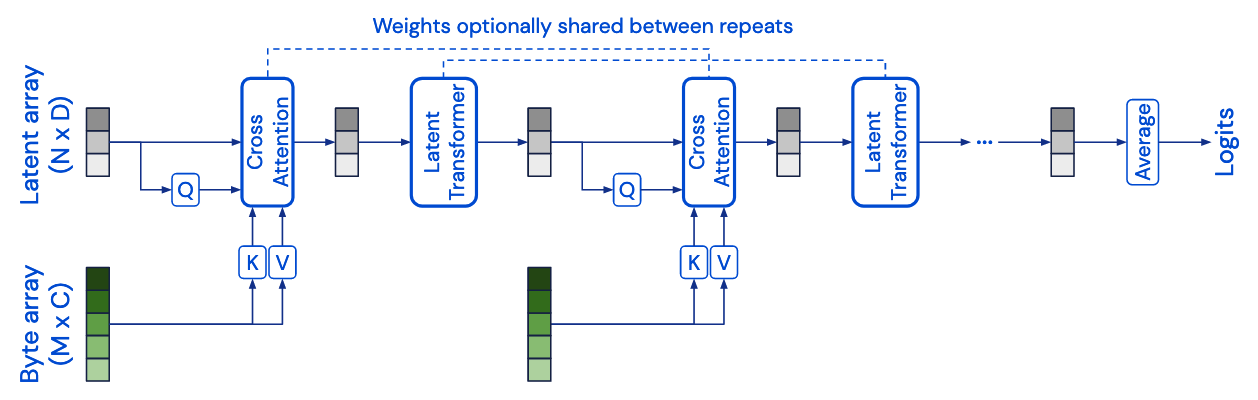
\includegraphics[width=\textwidth]{figures/figure_background_perceiver_architecture.png}
    \caption{The Perceiver is an architecture based on attentional principles that scales to high-dimensional inputs such as images, videos, audio, point-clouds, and multimodal combinations without making domain-specific assumptions. The Perceiver uses a cross-attention module to project an high-dimensional input byte array to a fixed-dimensional latent bottleneck (the number of input indices M is much larger than the number of latent indices $N$) before processing it using a deep stack of Transformer-style self-attention blocks in the latent space. The Perceiver iteratively attends to the input byte array by alternating cross-attention and latent self-attention blocks \cite{jaeglePerceiverGeneralPerception2021}.}
    \label{fig:figure_background_perceiver_architecture}
\end{figure}

The Perceiver architecture consists of two primary components: (i) a cross-attention module that maps an input byte array (e.g. a pixel array) and a latent array to an updated latent array, and (ii) a Transformer tower that maps this latent array to another latent array \cite{jaeglePerceiverGeneralPerception2021}. The Perceiver architecture is illustrated in Figure \ref{fig:figure_background_perceiver_architecture}. The model can be conceptualized as a recurrent neural network (RNN) unrolled in depth with the same input, rather than unrolled in time. A central challenge addressed by this architecture is the scaling of attention mechanisms to accommodate very large and diverse inputs. The Perceiver mitigates the quadratic complexity bottleneck inherent in standard Transformers by employing its cross-attention module. This module introduces an asymmetry into the attention operation when applied directly to the inputs.

Specifically, for a query $Q \in \mathbb{R}^{M \times D}$, key $K \in \mathbb{R}^{M \times C}$, and value $V \in \mathbb{R}^{M \times C}$ (where $C$ and $D$ represent channel dimensions), the computational complexity of the standard $QKV$ attention operation---formulated as $\text{softmax}(QK^T)V$---is $\mathcal{O}(M^2)$. This is due to matrix multiplications involving the large input index dimension $M$. The authors of Perceiver introduced an asymmetry: while $K$ and $V$ are projections of the input byte array (with $M$ elements), $Q$ is a projection of a learned latent array characterized by a much smaller index dimension $N \ll M$. The dimension $N$ of this latent array is a hyperparameter. Consequently, the resulting cross-attention operation exhibits a complexity of $\mathcal{O}(MN)$. It is important to note that within the Perceiver's cross-attention, linear projection layers are applied to generate $Q$, $K$, and $V$ such that they share a common channel dimension before the attention calculation.

This design enables Perceiver-based architectures to leverage significantly deeper Transformers compared to efficient Transformer variants that use linear complexity layers, without depending on domain-specific assumptions. Using $L$ to represent the number of layers in the Transformer tower, the complexity of a standard Transformer operating directly on $M$ input elements (bytes) can be represented as $\mathcal{O}(LM^2)$, whereas the complexity of Perceiver's latent Transformer (processing the $N$-dimensional latent array) is $\mathcal{O}(LN^2)$. Given that $N \ll M$, this substantially reduces the computational cost per layer. The overall architecture's complexity thus becomes $\mathcal{O}(MN + LN^2)$ for a latent Transformer with $L$ layers. This decoupling of the input size from the network depth is crucial, as it permits the addition of Transformer layers at a cost that is independent of the input size.

However, because the original Perceiver produced only one output per input, it was not as versatile as researchers required. Our proposed architecture aims to address this limitation by modifying the Perceiver architecture to make it akin to a recurrent unit processing input over time.


